\section{ModelHandlerTests} % (fold)
\label{prt:ModelHandlerTests}

\subsection{Test items} % (fold)
\label{sec:Test_items}

\begin{figure}[h!]
    \centerline{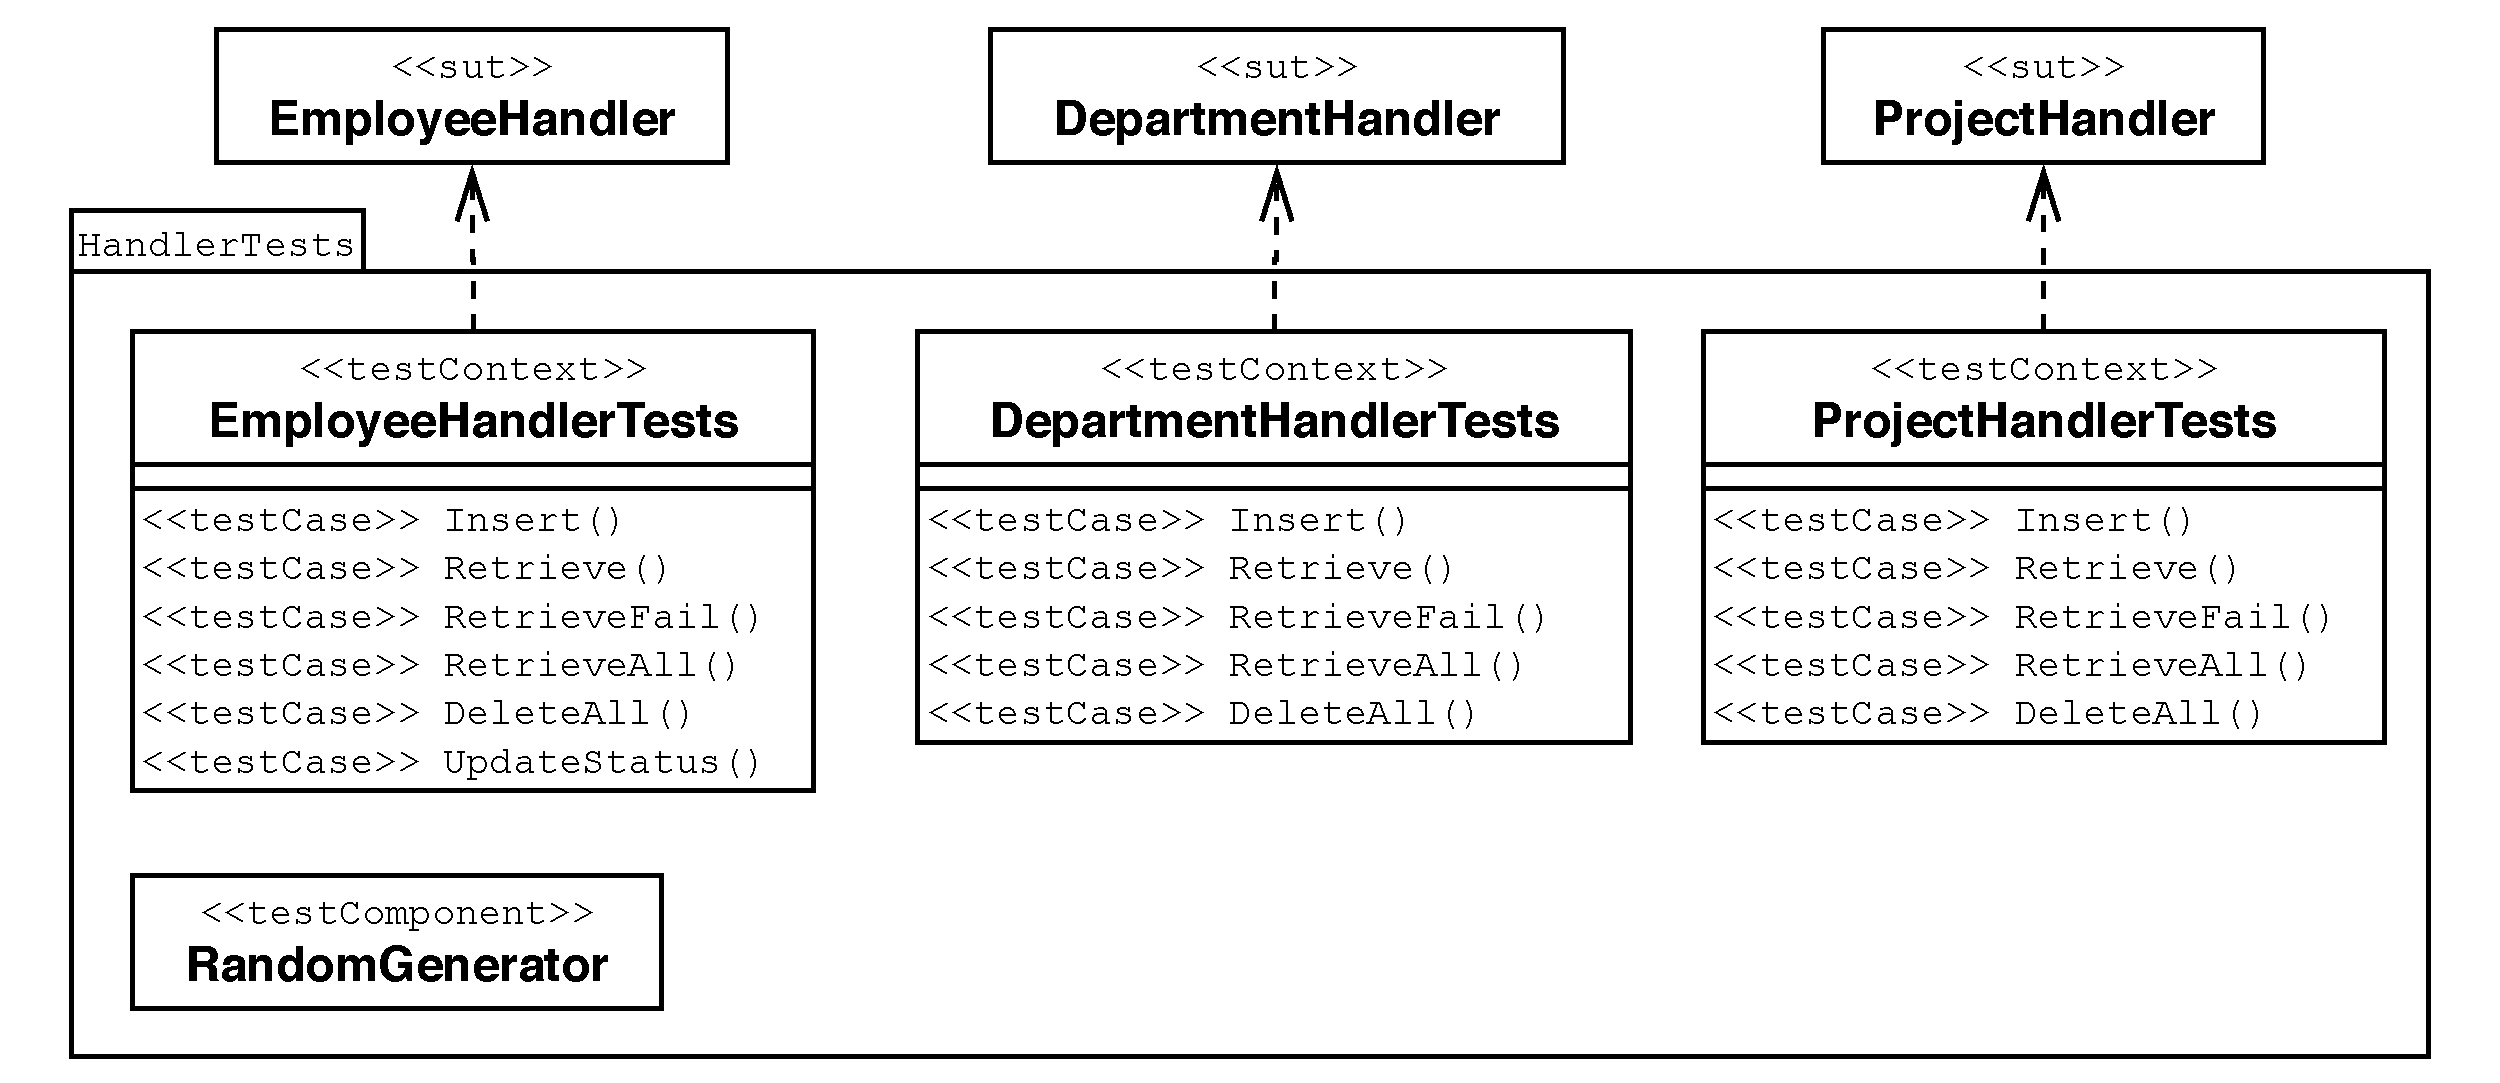
\includegraphics[width=1\textwidth]{tests_handler}}
    \caption{Test system for the S7Finder model handlers}
    \label{fig:test_system}
\end{figure}

This tests case covers the handlers for the model objects. These handlers
control the life cycle of all model objects, and are responsible for
caching them. All features of the handlers will be tested to ensure
expected behaviour. This includes the throwing of exceptions in error cases.
Random input is fed to the classes to ensure that all edge cases are found.

% subsection Test items (end)

\subsection{Input specifications} % (fold)
\label{sec:Input_specifications}

To ensure robust testing, all inputs are randomly generated. This includes
IDs for non-existant employees, and the values for randomly generated
employee, department and project objects. This enables us to think about
the conceptual operations the methods under testing perform, instead of
the specifics of one object.

% subsection Input specifications (end)

\subsection{Output specifications} % (fold)
\label{sec:Output_specifications}

Outputs from all methods are tested against the randomly generated values.
No transformations are made on the data, as all processing is done on the
gateway server. This enables simple output tests which contain logic that
is easy to validate.

% subsection Output specifications (end)

\subsection{Environmental needs} % (fold)
\label{sec:Environmental_needs}

As specified in the Test Plan, all tests must be run in the iOS Simulator through the
Monotouch port of NUnit.

% subsection Environmental needs (end)

% section Test case specification (end)

\clearpage

\section{DataSourceTests} % (fold)
\label{prt:DataSourceTests}

\subsection{Test items} % (fold)
\label{sec:Test_items}

\begin{figure}[h!]
    \centerline{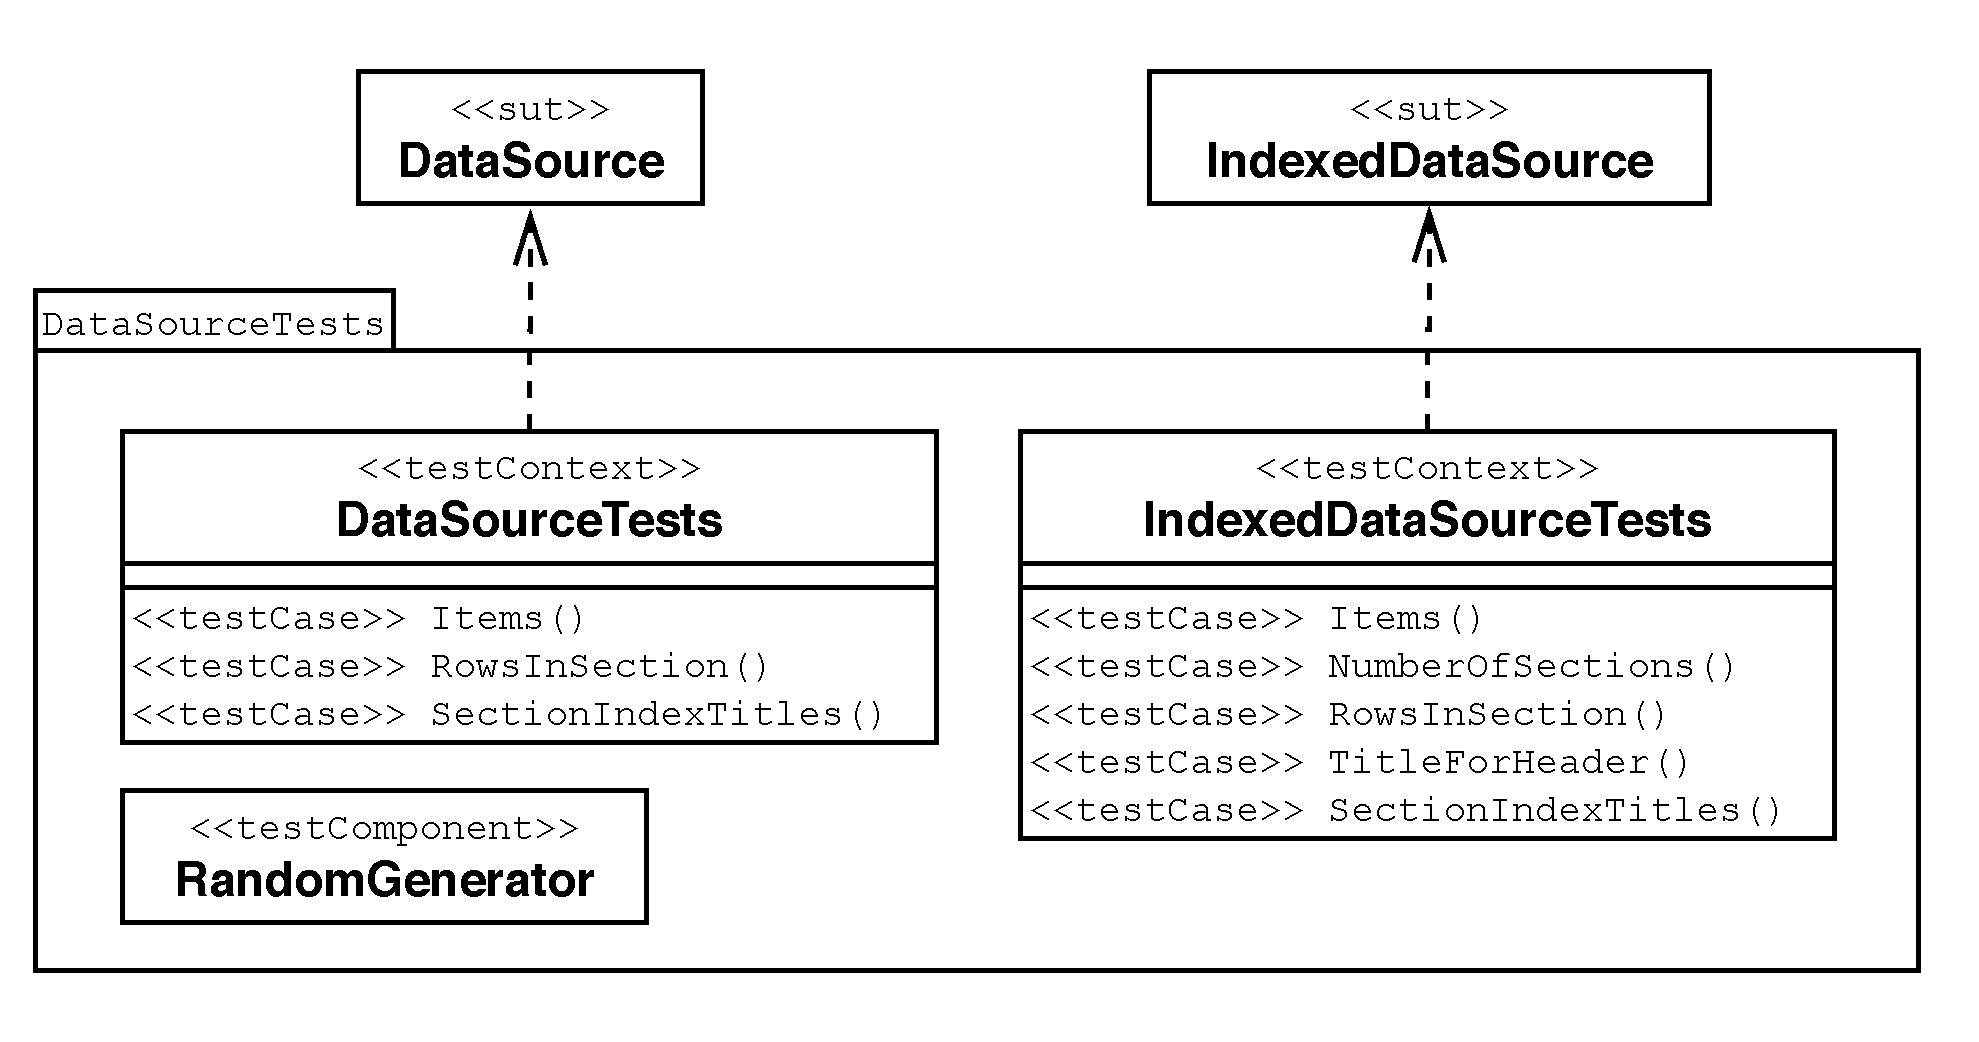
\includegraphics[width=1\textwidth]{tests_datasource}}
    \caption{Test system for the S7Finder data source}
    \label{fig:test_system}
\end{figure}

This tests case covers the datasource. The datasource maps data from
the model into the GUI tables defined by iOS. Only a limited subset of
the functionality can be tested due to the enormous amount of predefined
iOS methods inherited from the neccessary base classes. The scope of the
test will therefore be limited to the most basic functionality.

% subsection Test items (end)

\subsection{Input specifications} % (fold)
\label{sec:Input_specifications}

All testing is done using randomly generated IModelItems. The datasource only
holds these items in a predefined iOS format. It is therefore the execution of
the mapping concepts that are tested, and not specifics of an item list.

% subsection Input specifications (end)

\subsection{Output specifications} % (fold)
\label{sec:Output_specifications}

As all values are random, the output tests are made against the generated input.
All that must be ensured is that the items are grouped correctly, and that no
data is lost during the mapping.

% subsection Output specifications (end)

\subsection{Environmental needs} % (fold)
\label{sec:Environmental_needs}

As specified in the Test Plan, all tests must be run in the iOS Simulator through the
Monotouch port of NUnit.

% subsection Environmental needs (end)

% section DataSourceTests (end)

